% !TEX encoding = UTF-8 Unicode
%!TEX root = thesis.tex
% !TEX spellcheck = en-US
%%=========================================



\chapter{Background}

\section{Augmented Reality}
(Jentoft, 2020) AR can be defined as a system that fulfills three basic features: a combination of real and virtual worlds, real-time interaction, and accurate 3D registration of virtual and real objects.

\section{Graphics and Rendering}

\subsection*{Rasterization, Polygons and 3D models}

{
    \color{BrickRed}
    I feel that there is some misunderstanding about what a 3D model is.
    Maybe go in-depth about what I mean by 3D model. I have probably already used the term for different things.
}

\section{Neuro stuff}

\subsection*{Ethics of dissection}\label{chap:ethics}

\subsection*{The Waxholm Space Atlas of the Sprague Dawley Rat Brain}\label{chap:ratbrain}

{
    \color{BrickRed}
https://www.nitrc.org/projects/whs-sd-atlas
\begin{itemize}
    \item What is a atlas
    \item WHS and ratbrain is open, used and developed by NTNU St Olavs and UiO 
    \item Waxholm Space Atlas of the Sprague Dawley Rat Brain 
    \item Discuss difference between graphical 3D model and 3D atlas
\end{itemize}
}


%  In this pursuit we will also make use of high-resolution 3D imagery of a rat brain (see \autoref{chap:ratbrain}).  

This project makes use of high-resolution 3D-models of a rat brain. This brain model has been captured and manually delineated\footnotemark[1] by a collaboration between research groups at the University of Oslo and NTNU, and is in fact a highly accurate volumetric representations of the rat brain. This model is an open access community resource, intended as a free tool for education and research\footnotemark[2]. Within the convectional rasterization rendering pipe-line of Nevrolens, a polygonal asset derived from this volumetric model is naturally used. 

\footnotetext[1]{Delineation refers to the process of clearly defining different structures in the brain into separate namable parts.}
\footnotetext[2]{https://www.nitrc.org/projects/whs-sd-atlas}

The model is simply referred to as \textit{The Waxholm Space Atlas of the Sprague Dawley Rat Brain}. What follows is a brief explanation of each confusing part of the this name. 

\subsubsection*{Waxholm Space}\label{chap:whs}
\begin{wrapfigure}{R}{0.40\textwidth} 
    \centering
    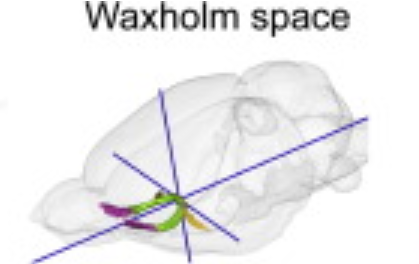
\includegraphics[width=0.30\textwidth]{fig/waxholmspace}
    \caption{\raggedright WHS \citep{WaxholmRatBrain2014}}
    \label{fig:waxholmspace}
\end{wrapfigure}

Waxholm Space (WHS) is a vector space defined as a standard reference space for the mouse brain and the rat brain \citep{WaxholmWithSimpleAbstract2013}. Its use as a coordinate system simplifies interoperability across atlases. It was developed by International Neuroinformatics Coordinating Facility (INCF) for the mouse brain, and has further been implemented in the rat brain by \citet{WaxholmRatBrain2014}. The following is the formal definition of WHS:


%  International Neuroinformatics Coordinating Facility (INCF) Digital Atlasing Project
\begin{quote}
\textit{
The coordinate system for WHS is defined as a continuous Cartesian system with the origin in the brain determined by 
\begin{itemize}
    \item the anterior commissure (AC) at the intersection between the mid sagittal plane,
    \item a coronal plane passing midway (rostro-caudal) through the anterior and posterior branches of AC, and
    \item a horizontal plane passing midway through the most dorsal and ventral aspect of the AC.
\end{itemize}
}
\citet{WaxholmSpaceAndMouseBrain2011}
\end{quote}

\noindent
\autoref{fig:waxholmspace} visualizes the axes through origin of WHS in the brain of a rat. Within the scope of this project WHS will be the local space of the rat brain model implemented in Nevrolens.

\subsubsection*{Brain Atlas}\label{chap:atlas}

A brain atlas is a composite representation based on one or more datasets of a given brain. An atlas generally has the function of highlighting some specified aspects and relations in the brain, and is a convectional tool in neuroscientific research \citep{Toga2000_AtlasBasics}. The convectional atlas is based on micrometer scale sliced sections in the brain, effectively creating two-dimensional layers through the brain. While functional, this "turns the brain into a book". Three-dimensional digital atlas are however relative newcomer on the neuro-imagery scene, by employing magnetic resonance imaging (MRI) and diffusion tensor imaging (DTI) the resulting atlases are complete volumetric representation of the subject brain \citep{WaxholmRatBrain2014}. 

This volumetric model is the basis for the delineated 3D-model used in Nevrolens.


\subsubsection*{Sprague Dawley}

Its a strain of laboratory rat.






\section{Related work}

\subsection*{HoloAnatomy}

\subsection*{Insight Heart}

\subsection*{SphenoBlock?}

\subsection*{Noe HoloCare stuff?}

